\newpage
\section{Modelli linari}
\subsection{Regression}
Un possibile esempio di regressione potrebbe essere un processo di stima di una funzione di valore
reale sulla base di un insieme finito di campioni rumorosi. Le conoscenze sarebbero $pairs(x, f(x) + random noise)$.\\
La task a questo punto sarebbe trovare $f$ per i dati nella seguente tabella.
\begin{figure}[h!]
    \centering
    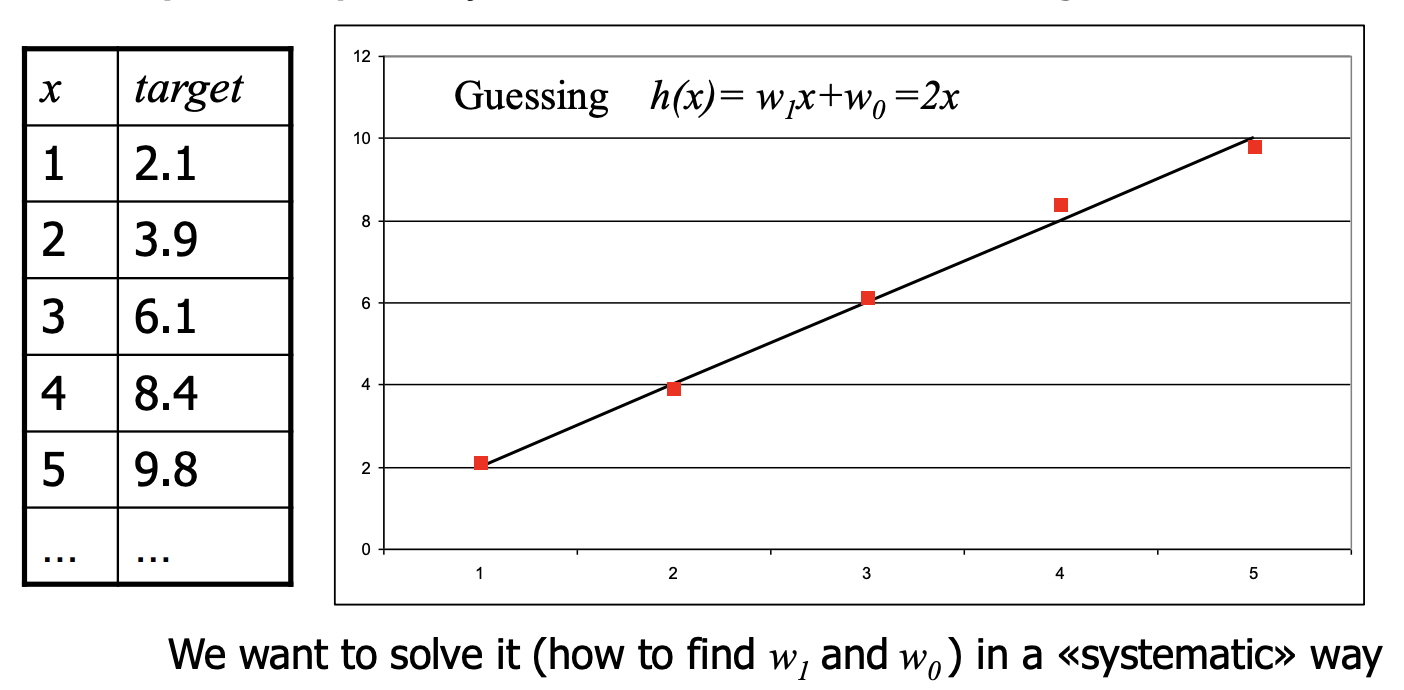
\includegraphics[width=0.65\textwidth]{images/esempio-regresione.png}
\end{figure}
\begin{example}
    Esempio di modelli linari:
    \begin{figure}[h!]
        \centering
        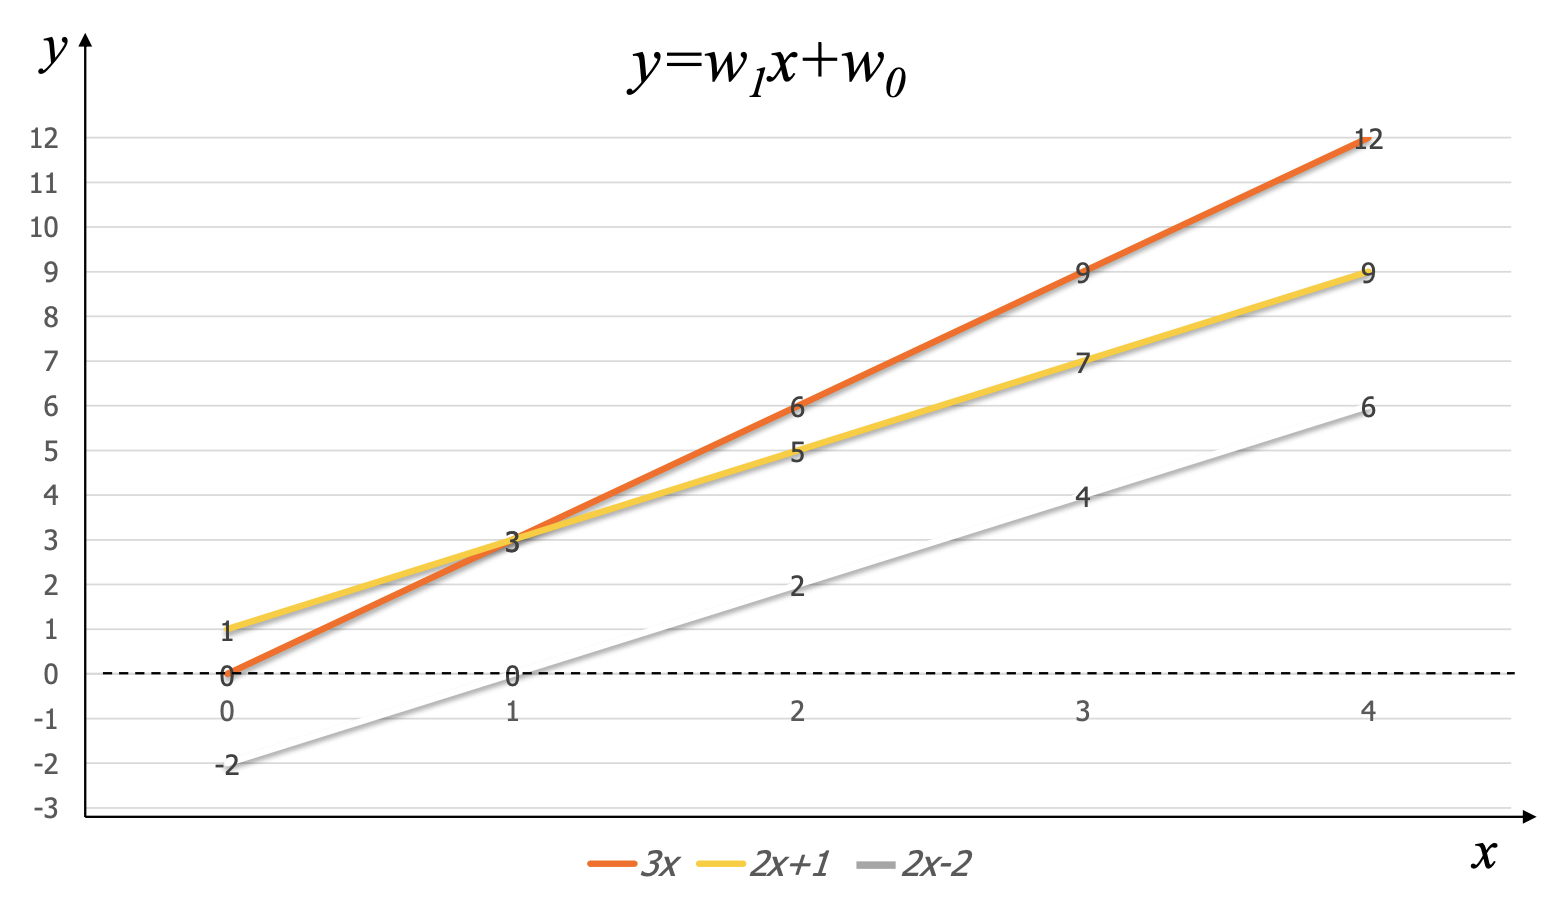
\includegraphics[width=0.65\textwidth]{images/esempio-modelli-lineari.png}
    \end{figure}
\end{example}

\subsubsection{Univariate linear regression}
Il caso univariante, semplice regressione linieare: iniziamo con 1 valore di inputl, $x$ e 
1 valore di output $y$.
\begin{definition}
    Assumiamo che un modello $h_w(x)$ espresso come:
    $$out = h(x) = w_1x + w_0$$
    dove $w$ è il coefficiente a valore reale/paramentro libero (peso).
\end{definition}
Si cerca di avere un adattamento dei dati secondo una “linea retta”. Trovare $h$ (modello lineare) che 
meglio si adattano ai dati (da gli insieme di dati osservati dei valori $x$ e $y$). Assumiamo che la variabile data (y) è (linearmente) 
associata ad un'altra viarialbe (x) o più variabili, da $y = w_1x + w_0 + noise$, dove $w$ è il free par e $noise$ è
un errore misurato al target (con una distribuzione normale). Andiamo a costruire un modello (trovare il valore $w$) per predirre/stimare il prezzo ($y$) dei punti
per altri (osservabile) valori $x$ (prediction).
\begin{figure}[h!]
    \centering
    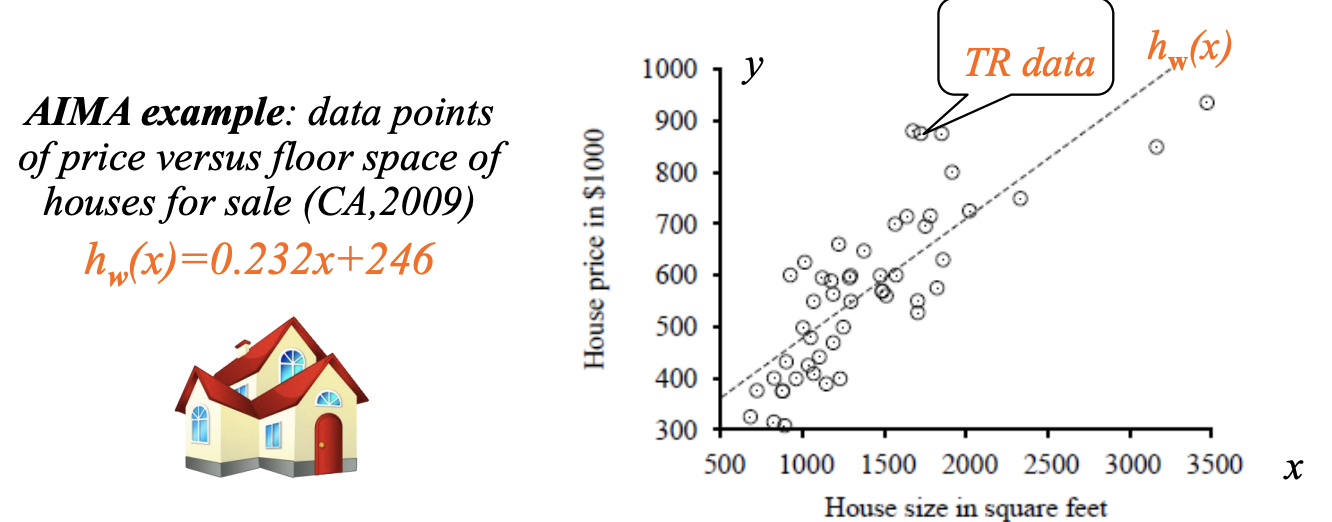
\includegraphics[width=0.55\textwidth]{images/task-model-esempio.png}
\end{figure}
Usiamo poi questi valori per \textbf{predirre/stimare} il prezzo (t) dei punti per altri valore osservabili.
\begin{figure}[h!]
    \centering
    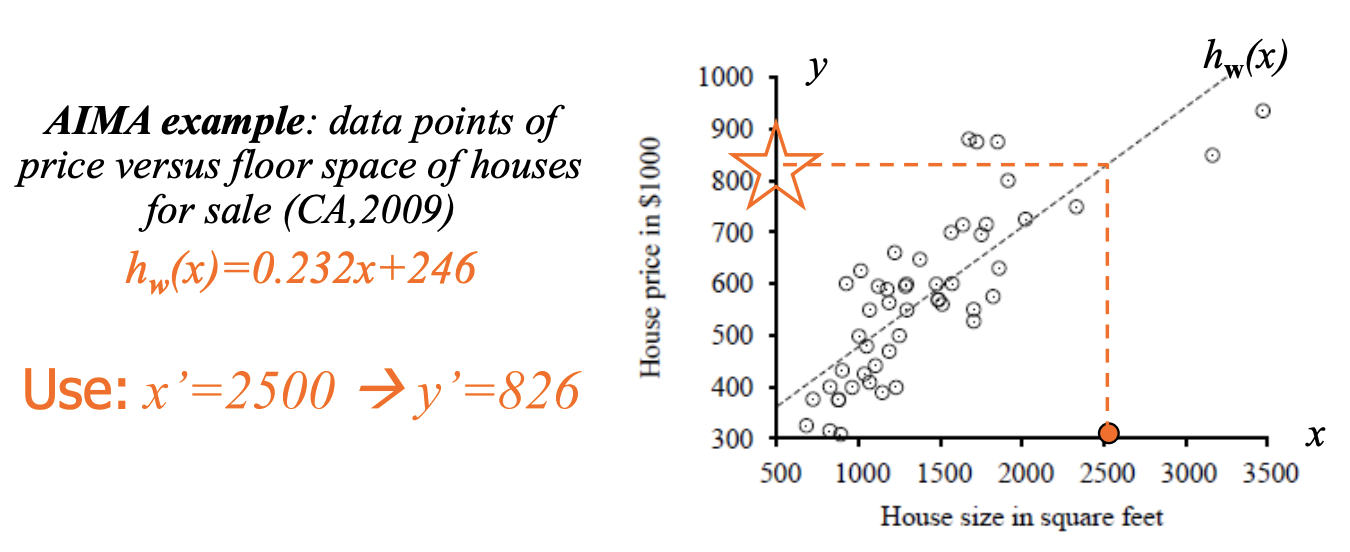
\includegraphics[width=0.55\textwidth]{images/uso-predizione-esempio.png}
\end{figure}

\subsubsection{Learning via LMS}
Abbiamo capito che quindi dobbiamo andare a trovare i valori dei paramentri $w$ ($w_1$ e $w_2$ nei casi univarianti) per andare a minimizzare 
l'output dell'errore del modello (per eseguire un buon fitting). In uno spazio di ipotesi infinito (valore $w$ continuo) abbiamo una buona soluzione
data dalla matematica classica, possiamo "imparare" da dei semplici tools, sebbene semplice incluse moltri concetti rileventi per
il ML moderno ed è alla abse dei metodi evoluti in the field. Definiamo qui una \textbf{funzione less / error} e usiamo il \textbf{Least Mean Square (LMS)} approccio.\\\\
\textbf{Il training} si fa trovando $w$ tale che minimizzi l'\textbf{errore}/la \textbf{perdita epirica} (il miglior dato che fitta nel training set con l'esempio $l$)

\begin{definition}
    Andiamo allora a definire LMS con:
    \begin{itemize}
        \item \textbf{Given} un insieme ti esempi di training $l$ ($x_p, y_p$) $p = 1 \dots l$
        \item \textbf{Trovare} $h_w(x)$ nella forma $w_1 x + w_0$ (quindi i valori di $w$) che minimizzano la perdita attesa dei dati di training.
    \end{itemize}
    Per la perdita usiamo la radice dell'errore.\\
    Da qui il \textbf{least (mean) square} si tratta di trovare la $w$ che minimizzi la somma residua delle ragdici [$argmin_w Error(w) in L_2$]
    $$Loss(h_w) = E(w) = \sum_{p=1}^{l} (y_p - h_w(x_p))^2 = \sum_{p=1}^{l}(y_p - (w_1 x_p + w_0))^2$$
    Dove $x_p$ è $p-th$ input/pattern/esample, $y_p$ l'output per $p$, $w$ free par., $l$ numero degli esempi.
\end{definition}
\hspace{-15pt}Perché usare LMS per adattarsi ai dati con $h$? Il \underline{least (mean) square} trova $w$ per minimizzare la \textbf{somma di radici residua} [$argmin_w Error(w) \in L_2$]:
\begin{figure}[h!]
    \centering
    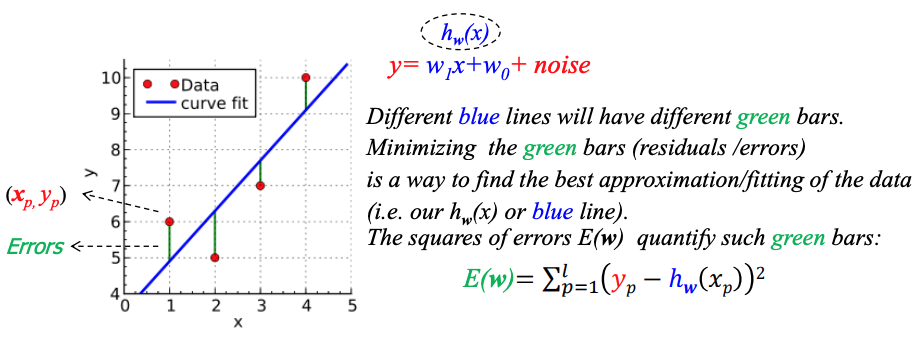
\includegraphics[width=0.6\textwidth]{images/lms.png}
\end{figure}

\hspace{-15pt}Il metodo dei minimi quadrati è un approccio standard alla soluzione approssimata di sistemi sovradeterminati, cioè insiemi di equazioni
in cui ci sono più equazioni che "sconociuti".\\\\
\textbf{Come si risolve?} Ricorda che il minimo locale è un punto stazionario, il gradiente è nullo.
$$\frac{\partial E(wi)}{\partial w_i} = 0 \hspace{15pt} i = 1, \dots, dim\_input + 1$$
Per una semplice regressione lineare (2 paramentri liberi) abbiamo che:
$$\frac{\partial E(w)}{\partial w_0} = 0 \hspace{15pt} \frac{\partial E(w)}{\partial w_1} = 0$$
Funzione di perdita convessa $\Rightarrow$ abbiamo la seguente soluzione (senza minimo locala).
$$w_1 = \frac{\sum x_p y_p - \frac{1}{l}\sum x_p \sum y_p}{\sum x_p^2 - \frac{1}{l} (\sum x_p^2)} = \frac{Conv[x, y]}{Var[x]}, \hspace{10pt} w_0 = \overline{y} - w_1 \overline{x} \hspace{20pt} \overline{y} = \frac{1}{l}\sum_{p \to 1} t_p  \hspace{7pt} \overline{x} = \frac{1}{l}\sum_{p\to 1}x_p$$
Calcolare il gradiante per 1 (ciascuno, omettendo quindi $p$ per $x$) pattern p. 
$$\frac{\partial E}{\partial w_i} = \frac{\partial (y - h_w(x))^2}{\partial w_i} = 2(y - h_w(x))\frac{\partial (y - h_w(h))}{\partial w_i} = 2(y - h_w(x))\frac{\partial (y - (w_1 x + w_0))}{\partial w_i}$$

\subsection{Summarizing}
\begin{itemize}
    \item \textbf{Given} un insieme di $l$ esempi di training ($x_p, y_p$) ed una funzione di perdita.
    \item \textbf{Find} il valore del peso $w$ per costruire $h_w(x)$ espresso come $y/out = w_1 x + w_0$ (minimizzare la perdita attesa dei dati di training)
\end{itemize}
\begin{figure}[h!]
    \centering
    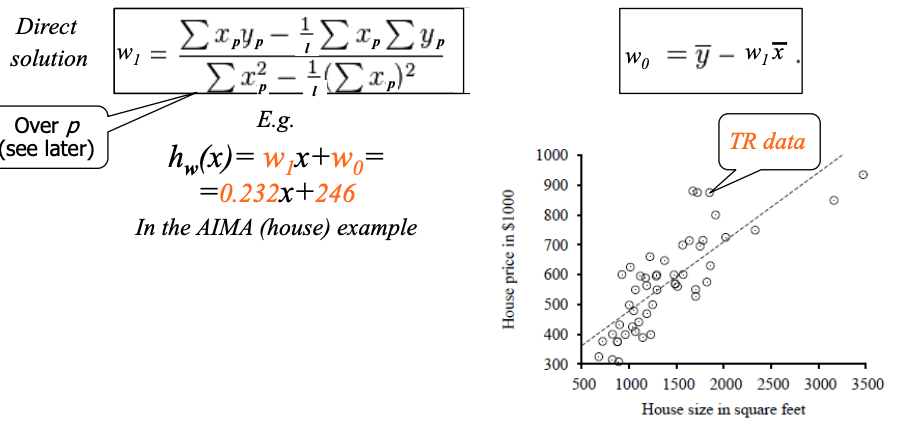
\includegraphics[width=0.55\textwidth]{images/summarizing.png}
\end{figure}
Ora è possibile usarlo per nuovi $x'$ per predirre $y'$. Vediamo ora un approccio differente.

\subsection{Gradiant descent (ricerca locale)}
Errore delle superfici per il linear model con 2 pesi. Parabolico per $E(w) = E([w_0, w_1]^T)$ (funzione quadratica convessa)
\begin{figure}[h!]
    \centering
    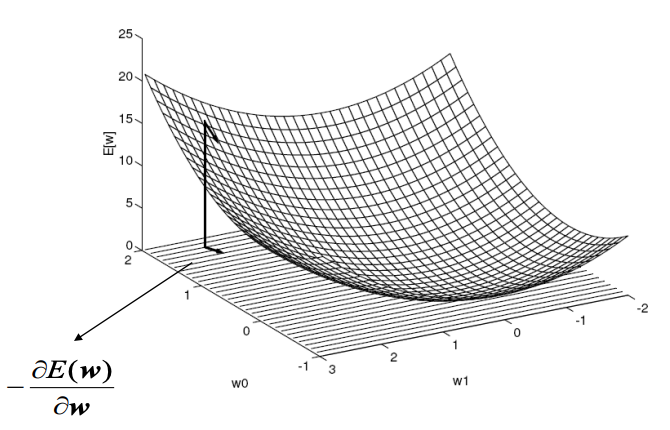
\includegraphics[width=0.4\textwidth]{images/error-surface.png}
\end{figure}

\hspace{-15pt}Spazio ipotetico con 2 parametri $w_0, w_1$. Il gradiente di $E(w)$ è il nostro "compasso" per trovare il minimo.\\\\
La derivazione precedente suggerisce la linea per costruire un \textbf{algoritmo iterativo} basato su $\frac{\partial E(w)}{\partial w_i}$
\begin{definition}
    \textbf{Gradiente} = direzione salita, possiamo muoverci verso il minimo con un gradiente in discesa ($\Delta w =$ gradiente di $E(w)$)
\end{definition}
\begin{definition}
    \textbf{ricerca locale} inizia con vettore di pesi iniziali. Esso viene modificato iterativamente per diminuire
    fino a minimizzare la funzione di errore (discesa più ripida).
    $$w_new = w + \eta \cdot \Delta w$$
    Dove $\eta$ è una constante (step size) chiamata \textbf{learning rate}
\end{definition}
\begin{figure}[h!]
    \centering
    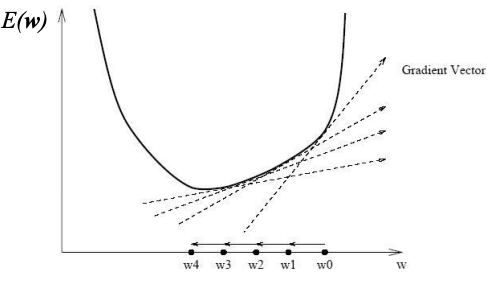
\includegraphics[width=0.5\textwidth]{images/gradieant-descent.png}
\end{figure}
Le motivazioni intuitive del gradiant descent sono che dalla formulazione, $w_new = w + \eta \cdot \Delta w$ possiamo ottenere:
$$\Delta w_0 = -\frac{\partial E(w)}{\partial w_0} = 2(y- h_w(x)) \hspace{15pt} \Delta w_1 = -\frac{\partial E(w)}{\partial w_i} = 2(y - h_w(x)) \cdot x$$
\begin{definition}
    Questa è una "error correction rule" chiamata \textbf{delta rule} che cambia la proporzione $w$ con l'errore (target-output):
    \begin{itemize}
        \item (target y - output) = err  = 0 $\to$ nessuna correzione 
        \item output > target $\to$ (y - h) < 0 (output troppo alto)
        \begin{itemize}
            \item Se $\Delta w_0$ negativo $\to$ si riduce $w_0$ e 
            \item if (input $x > 0$) $\Delta w_1$ negativo $\to$ si ricude $w_q$ else si aumenta $w_1$
        \end{itemize}
        \item output < target $\to$ $(y - h) > 0$ (output è troppo lento)
    \end{itemize} 
\end{definition}
\hspace{-15pt}In questo modo andiamo a migliorare l'apprendimento dai precedenti errori.\\\\
In conclusione possiamo dire che l'approccio del Gradiant descent è semplice ed efficacie per ricerca locale e approcci alla soluzione LMS, inoltre
ci permette di cercare in uno spazio infinito di ipotesi, può essere facilmente applicato sempre per $H$ contuno e perdite differenziabili non solo ai modelli lineari
(ess. reti neurali e deep learning models). A livello di efficienza molti miglioramenti sono possibili come il Newton's method, Conjugate Gradiant.
